\section{Client integrieren}
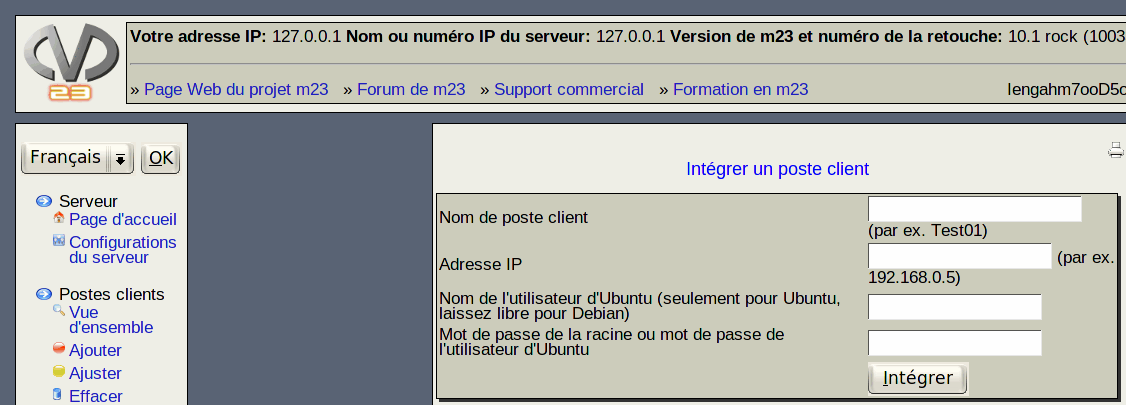
\includegraphics[scale=0.4]{/mdk/doc/manual/screenshots/de/client_assimilate.png} \\
Sie k�nnen bestehende Debian-Systeme mit m23 administrieren, indem Sie sie integrieren und somit m23 bekannt machen. F�r eine reibungslose Integration ist es erforderlich, da� der Client komplett hochgefahren und �ber das Netzwerk erreichbar ist. Nun werden nur noch drei Angaben ben�tigt:\\
\begin{itemize}
\item \textbf{Clientname}: Geben Sie hier einen Namen an, �ber den der Client im m23-Server verwaltet werden soll. Dieser Name mu� nicht zwangsl�ufig mit dem Hostnamen des Clients identisch sein.\\
\item \textbf{IP-Adresse}: Dies ist die (ggf. tempor�re) IP-Adresse des Clients.\\
\item \textbf{Name des Ubuntu-Benutzers (nur bei Ubuntu-Systemen, bei Debian leerlassen)}: Geben Sie hier einen Benutzernamen an, der auf dem Rechner ein Konto besitzt und mit dem man sich per SSH einloggen kann. Au�erdem mu� dieser Benutzer mittels sudo und seinem Pa�wort Befehle als root ausf�hren k�nnen. Dies wird nur bei Computern ben�tigt, auf denen Ubuntu installiert ist oder bei denen das Einloggen als root deaktiviert ist.\\
\item \textbf{Root-Pa�wort oder Pa�wort des Ubuntu-Benutzers}: Das aktuelle Root-Pa�wort des Clients bei Debian-Systemen oder das Pa�wort eines Benutzers bei Ubuntu-Systemen. Sie k�nnen dieses Feld allerdings auch leer lassen, wenn Sie eine manuelle Integration vorziehen.\\
\end{itemize}
Klicken Sie anschlie�end auf \textit{"Integrieren"}. Die Integration l�uft nun im Hintergrund.\\
\subsection{Hinweis}
F�r eine automatische Integration wird auf der Clientseite ein laufender SSH-D�mon, der das Einloggen als "root" erlaubt, sowie das Programm "wget" und das Paket "coreutils" vorrausgesetzt. Weiterhin ist es erforderlich, da� Pakete aus dem Internet per APT installiert werden k�nnen.\\
\subsection{Manuelle Integration}
Sollte auf dem Client kein SSH-D�mon laufen, so ist es auch m�glich, den Integrationsproze� auf dem Client per Hand anzusto�en. F�hren Sie dazu folgende Befehle als "root" in der Konsole des Clients aus (serverIP dabei durch die IP des m23-Servers ersetzen):\\
\begin{verbatim}
cd /tmp; wget http://$\langle$serverIP$\rangle$/work.php -O work.php; sh work.php
\end{verbatim}
\subsection{Hinweis f�r die Integration von Ubuntu-Systemen}
Ubuntusysteme lassen sich normalerweise nur manuell integrieren, da bei der Standardinstallation  kein laufender SSH-D�mon vorhanden ist. Starten Sie deshalb auf dem Ubuntu-Rechner eine Root-Konsole und beginnen Sie mit der manuellen Integration.\\
